%!TEX root = ../blob1.tex

\def\xxpar#1#2{\smallskip\noindent{\bf #1} {\it #2} \smallskip}

\section{$n$-categories}
\label{sec:ncats}

\subsection{Definition of $n$-categories}

Before proceeding, we need more appropriate definitions of $n$-categories, 
$A_\infty$ $n$-categories, modules for these, and tensor products of these modules.
(As is the case throughout this paper, by ``$n$-category" we implicitly intend some notion of
a `weak' $n$-category with `strong duality'.)

The definitions presented below tie the categories more closely to the topology
and avoid combinatorial questions about, for example, the minimal sufficient
collections of generalized associativity axioms; we prefer maximal sets of axioms to minimal sets.
For examples of topological origin, it is typically easy to show that they
satisfy our axioms.
For examples of a more purely algebraic origin, one would typically need the combinatorial
results that we have avoided here.

\medskip

Consider first ordinary $n$-categories.
We need a set (or sets) of $k$-morphisms for each $0\le k \le n$.
We must decide on the ``shape" of the $k$-morphisms.
Some $n$-category definitions model $k$-morphisms on the standard bihedron (interval, bigon, ...).
Other definitions have a separate set of 1-morphisms for each interval $[0,l] \sub \r$, 
a separate set of 2-morphisms for each rectangle $[0,l_1]\times [0,l_2] \sub \r^2$,
and so on.
(This allows for strict associativity.)
Still other definitions \nn{need refs for all these; maybe the Leinster book \cite{MR2094071}}
model the $k$-morphisms on more complicated combinatorial polyhedra.

We will allow our $k$-morphisms to have any shape, so long as it is homeomorphic to 
the standard $k$-ball.
In other words,

\begin{preliminary-axiom}{\ref{axiom:morphisms}}{Morphisms}
For any $k$-manifold $X$ homeomorphic 
to the standard $k$-ball, we have a set of $k$-morphisms
$\cC_k(X)$.
\end{preliminary-axiom}

Terminology: By ``a $k$-ball" we mean any $k$-manifold which is homeomorphic to the 
standard $k$-ball.
We {\it do not} assume that it is equipped with a 
preferred homeomorphism to the standard $k$-ball.
The same goes for ``a $k$-sphere" below.


Given a homeomorphism $f:X\to Y$ between $k$-balls (not necessarily fixed on 
the boundary), we want a corresponding
bijection of sets $f:\cC(X)\to \cC(Y)$.
(This will imply ``strong duality", among other things.)
So we replace the above with

\begin{axiom}[Morphisms]
\label{axiom:morphisms}
For each $0 \le k \le n$, we have a functor $\cC_k$ from 
the category of $k$-balls and 
homeomorphisms to the category of sets and bijections.
\end{axiom}


(Note: We usually omit the subscript $k$.)

We are so far  being deliberately vague about what flavor of manifolds we are considering.
They could be unoriented or oriented or Spin or $\mbox{Pin}_\pm$.
They could be topological or PL or smooth.
\nn{need to check whether this makes much difference --- see pseudo-isotopy below}
(If smooth, ``homeomorphism" should be read ``diffeomorphism", and we would need
to be fussier about corners.)
For each flavor of manifold there is a corresponding flavor of $n$-category.
We will concentrate of the case of PL unoriented manifolds.

Next we consider domains and ranges of morphisms (or, as we prefer to say, boundaries
of morphisms).
The 0-sphere is unusual among spheres in that it is disconnected.
Correspondingly, for 1-morphisms it makes sense to distinguish between domain and range.
(Actually, this is only true in the oriented case, with 1-morphsims parameterized
by oriented 1-balls.)
For $k>1$ and in the presence of strong duality the domain/range division makes less sense.
\nn{maybe say more here; rotate disk, Frobenius reciprocity blah blah}
We prefer to combine the domain and range into a single entity which we call the 
boundary of a morphism.
Morphisms are modeled on balls, so their boundaries are modeled on spheres:

\begin{axiom}[Boundaries (spheres)]
For each $0 \le k \le n-1$, we have a functor $\cC_k$ from 
the category of $k$-spheres and 
homeomorphisms to the category of sets and bijections.
\end{axiom}

(In order to conserve symbols, we use the same symbol $\cC_k$ for both morphisms and boundaries.)

\begin{axiom}[Boundaries (maps)]
For each $k$-ball $X$, we have a map of sets $\bd: \cC(X)\to \cC(\bd X)$.
These maps, for various $X$, comprise a natural transformation of functors.
\end{axiom}

(Note that the first ``$\bd$" above is part of the data for the category, 
while the second is the ordinary boundary of manifolds.)

Given $c\in\cC(\bd(X))$, let $\cC(X; c) \deq \bd^{-1}(c)$.

Most of the examples of $n$-categories we are interested in are enriched in the following sense.
The various sets of $n$-morphisms $\cC(X; c)$, for all $n$-balls $X$ and
all $c\in \cC(\bd X)$, have the structure of an object in some auxiliary category
(e.g.\ vector spaces, or modules over some ring, or chain complexes),
and all the structure maps of the $n$-category should be compatible with the auxiliary
category structure.
Note that this auxiliary structure is only in dimension $n$;
$\cC(Y; c)$ is just a plain set if $\dim(Y) < n$.

\medskip
\nn{
%At the moment I'm a little confused about orientations, and more specifically
%about the role of orientation-reversing maps of boundaries when gluing oriented manifolds.
Maybe need a discussion about what the boundary of a manifold with a 
structure (e.g. orientation) means.
Tentatively, I think we need to redefine the oriented boundary of an oriented $n$-manifold.
Instead of an ordinary oriented $(n-1)$-manifold via the inward (or outward) normal 
first (or last) convention, perhaps it is better to define the boundary to be an $(n-1)$-manifold
equipped with an orientation of its once-stabilized tangent bundle.
Similarly, in dimension $n-k$ we would have manifolds equipped with an orientation of 
their $k$ times stabilized tangent bundles.
(cf. [Stolz and Teichner].)
Probably should also have a framing of the stabilized dimensions in order to indicate which 
side the bounded manifold is on.
For the moment just stick with unoriented manifolds.}
\medskip

We have just argued that the boundary of a morphism has no preferred splitting into
domain and range, but the converse meets with our approval.
That is, given compatible domain and range, we should be able to combine them into
the full boundary of a morphism:

\begin{axiom}[Boundary from domain and range]
Let $S = B_1 \cup_E B_2$, where $S$ is a $k$-sphere $(0\le k\le n-1)$,
$B_i$ is a $k$-ball, and $E = B_1\cap B_2$ is a $k{-}1$-sphere (Figure \ref{blah3}).
Let $\cC(B_1) \times_{\cC(E)} \cC(B_2)$ denote the fibered product of the 
two maps $\bd: \cC(B_i)\to \cC(E)$.
Then we have an injective map
\[
	\gl_E : \cC(B_1) \times_{\cC(E)} \cC(B_2) \to \cC(S)
\]
which is natural with respect to the actions of homeomorphisms.
\end{axiom}

\begin{figure}[!ht]
$$
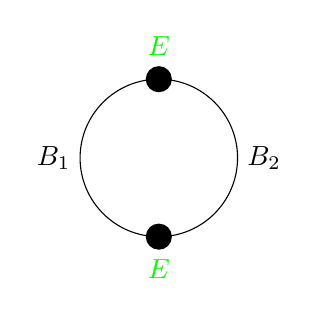
\begin{tikzpicture}[every label/.style={green}]
\node[fill=black, circle, label=below:$E$](S) at (0,0) {};
\node[fill=black, circle, label=above:$E$](N) at (0,2) {};
\draw (S) arc  (-90:90:1);
\draw (N) arc  (90:270:1);
\node[left] at (-1,1) {$B_1$};
\node[right] at (1,1) {$B_2$};
\end{tikzpicture}
$$
$$\mathfig{.4}{tempkw/blah3}$$
\caption{Combining two balls to get a full boundary}\label{blah3}\end{figure}

Note that we insist on injectivity above.

Let $\cC(S)_E$ denote the image of $\gl_E$.
We will refer to elements of $\cC(S)_E$ as ``splittable along $E$" or ``transverse to $E$". 

We will call the projection $\cC(S)_E \to \cC(B_i)$
a {\it restriction} map and write $\res_{B_i}(a)$
(or simply $\res(a)$ when there is no ambiguity), for $a\in \cC(S)_E$.
These restriction maps can be thought of as
domain and range maps, relative to the choice of splitting $S = B_1 \cup_E B_2$.

If $B$ is a $k$-ball and $E \sub \bd B$ splits $\bd B$ into two $k{-}1$-balls
as above, then we define $\cC(B)_E = \bd^{-1}(\cC(\bd B)_E)$.

Next we consider composition of morphisms.
For $n$-categories which lack strong duality, one usually considers
$k$ different types of composition of $k$-morphisms, each associated to a different direction.
(For example, vertical and horizontal composition of 2-morphisms.)
In the presence of strong duality, these $k$ distinct compositions are subsumed into 
one general type of composition which can be in any ``direction".

\begin{axiom}[Composition]
Let $B = B_1 \cup_Y B_2$, where $B$, $B_1$ and $B_2$ are $k$-balls ($0\le k\le n$)
and $Y = B_1\cap B_2$ is a $k{-}1$-ball (Figure \ref{blah5}).
Let $E = \bd Y$, which is a $k{-}2$-sphere.
Note that each of $B$, $B_1$ and $B_2$ has its boundary split into two $k{-}1$-balls by $E$.
We have restriction (domain or range) maps $\cC(B_i)_E \to \cC(Y)$.
Let $\cC(B_1)_E \times_{\cC(Y)} \cC(B_2)_E$ denote the fibered product of these two maps. 
Then (axiom) we have a map
\[
	\gl_Y : \cC(B_1)_E \times_{\cC(Y)} \cC(B_2)_E \to \cC(B)_E
\]
which is natural with respect to the actions of homeomorphisms, and also compatible with restrictions
to the intersection of the boundaries of $B$ and $B_i$.
If $k < n$ we require that $\gl_Y$ is injective.
(For $k=n$, see below.)
\end{axiom}

\begin{figure}[!ht]
$$\mathfig{.4}{tempkw/blah5}$$
\caption{From two balls to one ball}\label{blah5}\end{figure}

\begin{axiom}[Strict associativity]
The composition (gluing) maps above are strictly associative.
\end{axiom}

\begin{figure}[!ht]
$$\mathfig{.65}{tempkw/blah6}$$
\caption{An example of strict associativity}\label{blah6}\end{figure}

Notation: $a\bullet b \deq \gl_Y(a, b)$ and/or $a\cup b \deq \gl_Y(a, b)$.
In the other direction, we will call the projection from $\cC(B)_E$ to $\cC(B_i)_E$ 
a {\it restriction} map and write $\res_{B_i}(a)$ for $a\in \cC(B)_E$.
Compositions of boundary and restriction maps will also be called restriction maps.
For example, if $B$ is a $k$-ball and $Y\sub \bd B$ is a $k{-}1$-ball, there is a
restriction map from $\cC(B)_{\bd Y}$ to $\cC(Y)$.

%More notation and terminology:
%We will call the projection from $\cC(B)_E$ to $\cC(B_i)_E$ a {\it restriction}
%map

The above two axioms are equivalent to the following axiom,
which we state in slightly vague form.

\xxpar{Multi-composition:}
{Given any decomposition $B = B_1\cup\cdots\cup B_m$ of a $k$-ball
into small $k$-balls, there is a 
map from an appropriate subset (like a fibered product) 
of $\cC(B_1)\times\cdots\times\cC(B_m)$ to $\cC(B)$,
and these various $m$-fold composition maps satisfy an
operad-type strict associativity condition (Figure \ref{blah7}).}

\begin{figure}[!ht]
$$\mathfig{.8}{tempkw/blah7}$$
\caption{Operadish composition and associativity}\label{blah7}\end{figure}

The next axiom is related to identity morphisms, though that might not be immediately obvious.

\begin{axiom}[Product (identity) morphisms]
Let $X$ be a $k$-ball and $D$ be an $m$-ball, with $k+m \le n$.
Then we have a map $\cC(X)\to \cC(X\times D)$, usually denoted $a\mapsto a\times D$ for $a\in \cC(X)$.
If $f:X\to X'$ and $\tilde{f}:X\times D \to X'\times D'$ are maps such that the diagram
\[ \xymatrix{
	X\times D \ar[r]^{\tilde{f}} \ar[d]_{\pi} & X'\times D' \ar[d]^{\pi} \\
	X \ar[r]^{f} & X'
} \]
commutes, then we have 
\[
	\tilde{f}(a\times D) = f(a)\times D' .
\]
Product morphisms are compatible with gluing (composition) in both factors:
\[
	(a'\times D)\bullet(a''\times D) = (a'\bullet a'')\times D
\]
and
\[
	(a\times D')\bullet(a\times D'') = a\times (D'\bullet D'') .
\]
\nn{if pinched boundary, then remove first case above}
Product morphisms are associative:
\[
	(a\times D)\times D' = a\times (D\times D') .
\]
(Here we are implicitly using functoriality and the obvious homeomorphism
$(X\times D)\times D' \to X\times(D\times D')$.)
Product morphisms are compatible with restriction:
\[
	\res_{X\times E}(a\times D) = a\times E
\]
for $E\sub \bd D$ and $a\in \cC(X)$.
\end{axiom}

\nn{need even more subaxioms for product morphisms?}

\nn{Almost certainly we need a little more than the above axiom.
More specifically, in order to bootstrap our way from the top dimension
properties of identity morphisms to low dimensions, we need regular products,
pinched products and even half-pinched products.
I'm not sure what the best way to cleanly axiomatize the properties of these various
products is.
For the moment, I'll assume that all flavors of the product are at
our disposal, and I'll plan on revising the axioms later.}

\nn{current idea for fixing this: make the above axiom a ``preliminary version"
(as we have already done with some of the other axioms), then state the official
axiom for maps $\pi: E \to X$ which are almost fiber bundles.
one option is to restrict E to be a (full/half/not)-pinched product (up to homeo).
the alternative is to give some sort of local criterion for what's allowed.
state a gluing axiom for decomps $E = E'\cup E''$ where all three are of the correct type.
}

All of the axioms listed above hold for both ordinary $n$-categories and $A_\infty$ $n$-categories.
The last axiom (below), concerning actions of 
homeomorphisms in the top dimension $n$, distinguishes the two cases.

We start with the plain $n$-category case.

\begin{preliminary-axiom}{\ref{axiom:extended-isotopies}}{Isotopy invariance in dimension $n$}
Let $X$ be an $n$-ball and $f: X\to X$ be a homeomorphism which restricts
to the identity on $\bd X$ and is isotopic (rel boundary) to the identity.
Then $f$ acts trivially on $\cC(X)$; $f(a) = a$ for all $a\in \cC(X)$.
\end{preliminary-axiom}

This axiom needs to be strengthened to force product morphisms to act as the identity.
Let $X$ be an $n$-ball and $Y\sub\bd X$ be an $n{-}1$-ball.
Let $J$ be a 1-ball (interval).
We have a collaring homeomorphism $s_{Y,J}: X\cup_Y (Y\times J) \to X$.
(Here we use the ``pinched" version of $Y\times J$.
\nn{need notation for this})
We define a map
\begin{eqnarray*}
	\psi_{Y,J}: \cC(X) &\to& \cC(X) \\
	a & \mapsto & s_{Y,J}(a \cup ((a|_Y)\times J)) .
\end{eqnarray*}
(See Figure \ref{glue-collar}.)
\begin{figure}[!ht]
\begin{equation*}
\begin{tikzpicture}
\def\rad{1}
\def\srad{0.75}
\def\gap{4.5}
\foreach \i in {0, 1, 2} {
	\node(\i) at ($\i*(\gap,0)$) [draw, circle through = {($\i*(\gap,0)+(\rad,0)$)}] {};
	\node(\i-small) at (\i.east) [circle through={($(\i.east)+(\srad,0)$)}] {};
	\foreach \n in {1,2} {
		\fill (intersection \n of \i-small and \i) node(\i-intersection-\n) {} circle (2pt);
	}
}

\begin{scope}[decoration={brace,amplitude=10,aspect=0.5}]
	\draw[decorate] (0-intersection-1.east) -- (0-intersection-2.east);
\end{scope}
\node[right=1mm] at (0.east) {$a$};
\draw[->] ($(0.east)+(0.75,0)$) -- ($(1.west)+(-0.2,0)$);

\draw (1-small)  circle (\srad);
\foreach \theta in {90, 72, ..., -90} {
	\draw[blue] (1) -- ($(1)+(\rad,0)+(\theta:\srad)$);
}
\filldraw[fill=white] (1) circle (\rad);
\foreach \n in {1,2} {
	\fill (intersection \n of 1-small and 1) circle (2pt);
}
\node[below] at (1-small.south) {$a \times J$};
\draw[->] ($(1.east)+(1,0)$) -- ($(2.west)+(-0.2,0)$);

\begin{scope}
\path[clip] (2) circle (\rad);
\draw[clip] (2.east) circle (\srad);
\foreach \y in {1, 0.86, ..., -1} {
	\draw[blue] ($(2)+(-1,\y) $)-- ($(2)+(1,\y)$);
}
\end{scope}
\end{tikzpicture}
\end{equation*}
\begin{equation*}
\xymatrix@C+2cm{\cC(X) \ar[r]^(0.45){\text{glue}} & \cC(X \cup \text{collar}) \ar[r]^(0.55){\text{homeo}} & \cC(X)}
\end{equation*}

\caption{Extended homeomorphism.}\label{glue-collar}\end{figure}
We say that $\psi_{Y,J}$ is {\it extended isotopic} to the identity map.
\nn{bad terminology; fix it later}
\nn{also need to make clear that plain old isotopic to the identity implies
extended isotopic}
\nn{maybe remark that in some examples (e.g.\ ones based on sub cell complexes) 
extended isotopies are also plain isotopies, so
no extension necessary}
It can be thought of as the action of the inverse of
a map which projects a collar neighborhood of $Y$ onto $Y$.

The revised axiom is

\stepcounter{axiom}
\begin{axiom-numbered}{\arabic{axiom}a}{Extended isotopy invariance in dimension $n$}
\label{axiom:extended-isotopies}
Let $X$ be an $n$-ball and $f: X\to X$ be a homeomorphism which restricts
to the identity on $\bd X$ and is extended isotopic (rel boundary) to the identity.
Then $f$ acts trivially on $\cC(X)$.
\end{axiom-numbered}

\nn{need to rephrase this, since extended isotopies don't correspond to homeomorphisms.}

\smallskip

For $A_\infty$ $n$-categories, we replace
isotopy invariance with the requirement that families of homeomorphisms act.
For the moment, assume that our $n$-morphisms are enriched over chain complexes.

\begin{axiom-numbered}{\arabic{axiom}b}{Families of homeomorphisms act in dimension $n$}
For each $n$-ball $X$ and each $c\in \cC(\bd X)$ we have a map of chain complexes
\[
	C_*(\Homeo_\bd(X))\ot \cC(X; c) \to \cC(X; c) .
\]
Here $C_*$ means singular chains and $\Homeo_\bd(X)$ is the space of homeomorphisms of $X$
which fix $\bd X$.
These action maps are required to be associative up to homotopy
\nn{iterated homotopy?}, and also compatible with composition (gluing) in the sense that
a diagram like the one in Proposition \ref{CDprop} commutes.
\nn{repeat diagram here?}
\nn{restate this with $\Homeo(X\to X')$?  what about boundary fixing property?}
\end{axiom-numbered}

We should strengthen the above axiom to apply to families of extended homeomorphisms.
To do this we need to explain how extended homeomorphisms form a topological space.
Roughly, the set of $n{-}1$-balls in the boundary of an $n$-ball has a natural topology,
and we can replace the class of all intervals $J$ with intervals contained in $\r$.
\nn{need to also say something about collaring homeomorphisms.}
\nn{this paragraph needs work.}

Note that if we take homology of chain complexes, we turn an $A_\infty$ $n$-category
into a plain $n$-category (enriched over graded groups).
\nn{say more here?}
In the other direction, if we enrich over topological spaces instead of chain complexes,
we get a space version of an $A_\infty$ $n$-category, with $\Homeo_\bd(X)$ acting 
instead of  $C_*(\Homeo_\bd(X))$.
Taking singular chains converts a space-type $A_\infty$ $n$-category into a chain complex
type $A_\infty$ $n$-category.

\medskip

The alert reader will have already noticed that our definition of (plain) $n$-category
is extremely similar to our definition of topological fields.
The main difference is that for the $n$-category definition we restrict our attention to balls
(and their boundaries), while for fields we consider all manifolds.
(A minor difference is that in the category definition we directly impose isotopy
invariance in dimension $n$, while in the fields definition we have non-isotopy-invariant fields
but then mod out by local relations which imply isotopy invariance.)
Thus a system of fields determines an $n$-category simply by restricting our attention to
balls.
This $n$-category can be thought of as the local part of the fields.
Conversely, given an $n$-category we can construct a system of fields via 
a colimit construction; see below.

%\nn{Next, say something about $A_\infty$ $n$-categories and ``homological" systems
%of fields.
%The universal (colimit) construction becomes our generalized definition of blob homology.
%Need to explain how it relates to the old definition.}

\medskip

\subsection{Examples of $n$-categories}

\nn{these examples need to be fleshed out a bit more}

We know describe several classes of examples of $n$-categories satisfying our axioms.

\begin{example}{Maps to a space}
\label{ex:maps-to-a-space}%
Fix $F$ a closed $m$-manifold (keep in mind the case where $F$ is a point). Fix a `target space' $T$, any topological space.
For $X$ a $k$-ball or $k$-sphere with $k < n$, define $\cC(X)$ to be the set of 
all maps from $X\times F$ to $T$.
For $X$ an $n$-ball define $\cC(X)$ to be maps from $X\times F$ to $T$ modulo
homotopies fixed on $\bd X \times F$.
(Note that homotopy invariance implies isotopy invariance.)
For $a\in \cC(X)$ define the product morphism $a\times D \in \cC(X\times D)$ to
be $a\circ\pi_X$, where $\pi_X : X\times D \to X$ is the projection.
\end{example}

\begin{example}{Linearized, twisted, maps to a space}
\label{ex:linearized-maps-to-a-space}%
We can linearize the above example as follows.
Let $\alpha$ be an $(n{+}m{+}1)$-cocycle on $T$ with values in a ring $R$
(e.g.\ the trivial cocycle).
For $X$ of dimension less than $n$ define $\cC(X)$ as before.
For $X$ an $n$-ball and $c\in \cC(\bd X)$ define $\cC(X; c)$ to be
the $R$-module of finite linear combinations of maps from $X\times F$ to $T$,
modulo the relation that if $a$ is homotopic to $b$ (rel boundary) via a homotopy
$h: X\times F\times I \to T$, then $a \sim \alpha(h)b$.
\nn{need to say something about fundamental classes, or choose $\alpha$ carefully}
\end{example}

\begin{itemize}

\item \nn{Continue converting these into examples}

\item Given a traditional $n$-category $C$ (with strong duality etc.),
define $\cC(X)$ (with $\dim(X) < n$) 
to be the set of all $C$-labeled sub cell complexes of $X$.
(See Subsection \ref{sec:fields}.)
For $X$ an $n$-ball and $c\in \cC(\bd X)$, define $\cC(X)$ to finite linear
combinations of $C$-labeled sub cell complexes of $X$
modulo the kernel of the evaluation map.
Define a product morphism $a\times D$ to be the product of the cell complex of $a$ with $D$,
and with the same labeling as $a$.
More generally, start with an $n{+}m$-category $C$ and a closed $m$-manifold $F$.
Define $\cC(X)$, for $\dim(X) < n$,
to be the set of all $C$-labeled sub cell complexes of $X\times F$.
Define $\cC(X; c)$, for $X$ an $n$-ball,
to be the dual Hilbert space $A(X\times F; c)$.
\nn{refer elsewhere for details?}

\item Variation on the above examples:
We could allow $F$ to have boundary and specify boundary conditions on $X\times \bd F$,
for example product boundary conditions or take the union over all boundary conditions.
%\nn{maybe should not emphasize this case, since it's ``better" in some sense
%to think of these guys as affording a representation
%of the $n{+}1$-category associated to $\bd F$.}

\item Here's our version of the bordism $n$-category.
For a $k$-ball $X$, $k<n$, define $\cC(X)$ to be the set of all $k$-dimensional
submanifolds $W$ of $X\times \r^\infty$ such that the projection $W \to X$ is transverse
to $\bd X$.
For $k=n$ define $\cC(X)$ to be homeomorphism classes (rel boundary) of such submanifolds;
we identify $W$ and $W'$ if $\bd W = \bd W'$ and there is a homeomorphism
$W\to W'$ which restricts to the identity on the boundary.

\item \nn{sphere modules; ref to below}

\end{itemize}


We have two main examples of $A_\infty$ $n$-categories, coming from maps to a target space and from the blob complex.

\begin{example}{Chains of maps to a space}
We can modify Example \ref{ex:maps-to-a-space} above by defining $\cC(X; c)$ for an $n$-ball $X$  to be the chain complex 
$C_*(\Maps_c(X\times F \to T))$, where $\Maps_c$ denotes continuous maps restricting to $c$ on the boundary,
and $C_*$ denotes singular chains.
\end{example}

\begin{example}{Blob complexes of balls (with a fiber)}
Fix an $m$-dimensional manifold $F$.
Given a plain $n$-category $C$, 
when $X$ is a $k$-ball or $k$-sphere, with $k<n-m$, define $\cC(X) = C(X)$. When $X$ is an $(n-m)$-ball,
define $\cC(X; c) = \bc^C_*(X\times F; c)$
where $\bc^C_*$ denotes the blob complex based on $C$.
\end{example}

\begin{defn}
\nn{should add $\infty$ version of bordism $n$-cat}
\end{defn}






\subsection{From $n$-categories to systems of fields}
\label{ss:ncat_fields}

We can extend the functors $\cC$ above from $k$-balls to arbitrary $k$-manifolds as follows.

Let $W$ be a $k$-manifold, $1\le k \le n$.
We will define a set $\cC(W)$.
(If $k = n$ and our $k$-categories are enriched, then
$\cC(W)$ will have additional structure; see below.)
$\cC(W)$ will be the colimit of a functor defined on a category $\cJ(W)$,
which we define next.

Define a permissible decomposition of $W$ to be a cell decomposition
\[
	W = \bigcup_a X_a ,
\]
where each closed top-dimensional cell $X_a$ is an embedded $k$-ball.
Given permissible decompositions $x$ and $y$, we say that $x$ is a refinement
of $y$, or write $x \le y$, if each ball of $y$ is a union of balls of $x$.
This defines a partial ordering $\cJ(W)$, which we will think of as a category.
(The objects of $\cJ(W)$ are permissible decompositions of $W$, and there is a unique
morphism from $x$ to $y$ if and only if $x$ is a refinement of $y$.
See Figure \ref{partofJfig}.)

\begin{figure}[!ht]
\begin{equation*}
\mathfig{.63}{tempkw/zz2}
\end{equation*}
\caption{A small part of $\cJ(W)$}
\label{partofJfig}
\end{figure}


$\cC$ determines 
a functor $\psi_\cC$ from $\cJ(W)$ to the category of sets 
(possibly with additional structure if $k=n$).
For a decomposition $x = (X_a)$ in $\cJ(W)$, define $\psi_\cC(x)$ to be the subset
\[
	\psi_\cC(x) \sub \prod_a \cC(X_a)
\]
such that the restrictions to the various pieces of shared boundaries amongst the
$X_a$ all agree.
(Think fibered product.)
If $x$ is a refinement of $y$, define a map $\psi_\cC(x)\to\psi_\cC(y)$
via the composition maps of $\cC$.
(If $\dim(W) = n$ then we need to also make use of the monoidal
product in the enriching category.
\nn{should probably be more explicit here})

Finally, define $\cC(W)$ to be the colimit of $\psi_\cC$.
When $k<n$ or $k=n$ and we are in the plain (non-$A_\infty$) case, this means that
for each decomposition $x$ there is a map
$\psi_\cC(x)\to \cC(W)$, these maps are compatible with the refinement maps
above, and $\cC(W)$ is universal with respect to these properties.
When $k=n$ and we are in the $A_\infty$ case, it means
homotopy colimit.

More concretely, in the plain case enriched over vector spaces, and with $\dim(W) = n$, we can take
\[
	\cC(W) = \left( \oplus_x \psi_\cC(x)\right) \big/ K
\]
where $K$ is generated by all things of the form $a - g(a)$, where
$a\in \psi_\cC(x)$ for some decomposition $x$, $x\le y$, and $g: \psi_\cC(x)
\to \psi_\cC(y)$ is value of $\psi_\cC$ on the antirefinement $x\to y$.

In the $A_\infty$ case enriched over chain complexes, the concrete description of the colimit
is as follows.
%\nn{should probably rewrite this to be compatible with some standard reference}
Define an $m$-sequence to be a sequence $x_0 \le x_1 \le \dots \le x_m$ of permissible decompositions.
Such sequences (for all $m$) form a simplicial set.
Let
\[
	V = \bigoplus_{(x_i)} \psi_\cC(x_0) ,
\]
where the sum is over all $m$-sequences and all $m$, and each summand is degree shifted by $m$.
We endow $V$ with a differential which is the sum of the differential of the $\psi_\cC(x_0)$
summands plus another term using the differential of the simplicial set of $m$-sequences.
More specifically, if $(a, \bar{x})$ denotes an element in the $\bar{x}$
summand of $V$ (with $\bar{x} = (x_0,\dots,x_k)$), define
\[
	\bd (a, \bar{x}) = (\bd a, \bar{x}) \pm (g(a), d_0(\bar{x})) + \sum_{j=1}^k \pm (a, d_j(\bar{x})) ,
\]
where $d_j(\bar{x}) = (x_0,\dots,x_{j-1},x_{j+1},\dots,x_k)$ and $g: \psi_\cC(x_0)\to \psi_\cC(x_1)$
is the usual map.
\nn{need to say this better}
\nn{maybe mention that there is a version that emphasizes minimal gluings (antirefinements) which
combine only two balls at a time; for $n=1$ this version will lead to usual definition
of $A_\infty$ category}

We will call $m$ the filtration degree of the complex.
We can think of this construction as starting with a disjoint copy of a complex for each
permissible decomposition (filtration degree 0).
Then we glue these together with mapping cylinders coming from gluing maps
(filtration degree 1).
Then we kill the extra homology we just introduced with mapping cylinder between the mapping cylinders (filtration degree 2).
And so on.

$\cC(W)$ is functorial with respect to homeomorphisms of $k$-manifolds.

It is easy to see that
there are well-defined maps $\cC(W)\to\cC(\bd W)$, and that these maps
comprise a natural transformation of functors.

\nn{need to finish explaining why we have a system of fields;
need to say more about ``homological" fields? 
(actions of homeomorphisms);
define $k$-cat $\cC(\cdot\times W)$}



\subsection{Modules}

Next we define [$A_\infty$] $n$-category modules (a.k.a.\ representations,
a.k.a.\ actions).
The definition will be very similar to that of $n$-categories.
\nn{** need to make sure all revisions of $n$-cat def are also made to module def.}
\nn{should they be called $n$-modules instead of just modules?  probably not, but worth considering.}

Our motivating example comes from an $(m{-}n{+}1)$-dimensional manifold $W$ with boundary
in the context of an $m{+}1$-dimensional TQFT.
Such a $W$ gives rise to a module for the $n$-category associated to $\bd W$.
This will be explained in more detail as we present the axioms.

Fix an $n$-category $\cC$.

Define a {\it marked $k$-ball} to be a pair $(B, N)$ homeomorphic to the pair
(standard $k$-ball, northern hemisphere in boundary of standard $k$-ball).
We call $B$ the ball and $N$ the marking.
A homeomorphism between marked $k$-balls is a homeomorphism of balls which
restricts to a homeomorphism of markings.

\xxpar{Module morphisms}
{For each $0 \le k \le n$, we have a functor $\cM_k$ from 
the category of marked $k$-balls and 
homeomorphisms to the category of sets and bijections.}

(As with $n$-categories, we will usually omit the subscript $k$.)

For example, let $\cD$ be the $m{+}1$-dimensional TQFT which assigns to a $k$-manifold $N$ the set 
of maps from $N$ to $T$, modulo homotopy (and possibly linearized) if $k=m$.
Let $W$ be an $(m{-}n{+}1)$-dimensional manifold with boundary.
Let $\cC$ be the $n$-category with $\cC(X) \deq \cD(X\times \bd W)$.
Let $\cM(B, N) \deq \cD((B\times \bd W)\cup (N\times W))$.
(The union is along $N\times \bd W$.)
(If $\cD$ were a general TQFT, we would define $\cM(B, N)$ to be
the subset of $\cD((B\times \bd W)\cup (N\times W))$ which is splittable along $N\times \bd W$.)

\begin{figure}[!ht]
$$\mathfig{.8}{tempkw/blah15}$$
\caption{From manifold with boundary collar to marked ball}\label{blah15}\end{figure}

Define the boundary of a marked $k$-ball $(B, N)$ to be the pair $(\bd B \setmin N, \bd N)$.
Call such a thing a {marked $k{-}1$-hemisphere}.

\xxpar{Module boundaries, part 1:}
{For each $0 \le k \le n-1$, we have a functor $\cM_k$ from 
the category of marked $k$-hemispheres and 
homeomorphisms to the category of sets and bijections.}

In our example, let $\cM(H) \deq \cD(H\times\bd W \cup \bd H\times W)$.

\xxpar{Module boundaries, part 2:}
{For each marked $k$-ball $M$ we have a map of sets $\bd: \cM(M)\to \cM(\bd M)$.
These maps, for various $M$, comprise a natural transformation of functors.}

Given $c\in\cM(\bd M)$, let $\cM(M; c) \deq \bd^{-1}(c)$.

If the $n$-category $\cC$ is enriched over some other category (e.g.\ vector spaces),
then $\cM(M; c)$ should be an object in that category for each marked $n$-ball $M$
and $c\in \cC(\bd M)$.

\xxpar{Module domain $+$ range $\to$ boundary:}
{Let $H = M_1 \cup_E M_2$, where $H$ is a marked $k$-hemisphere ($0\le k\le n-1$),
$M_i$ is a marked $k$-ball, and $E = M_1\cap M_2$ is a marked $k{-}1$-hemisphere.
Let $\cM(M_1) \times_{\cM(E)} \cM(M_2)$ denote the fibered product of the 
two maps $\bd: \cM(M_i)\to \cM(E)$.
Then (axiom) we have an injective map
\[
	\gl_E : \cM(M_1) \times_{\cM(E)} \cM(M_2) \to \cM(H)
\]
which is natural with respect to the actions of homeomorphisms.}

Let $\cM(H)_E$ denote the image of $\gl_E$.
We will refer to elements of $\cM(H)_E$ as ``splittable along $E$" or ``transverse to $E$". 


\xxpar{Axiom yet to be named:}
{For each marked $k$-hemisphere $H$ there is a restriction map
$\cM(H)\to \cC(H)$.  
($\cC(H)$ means apply $\cC$ to the underlying $k$-ball of $H$.)
These maps comprise a natural transformation of functors.}

Note that combining the various boundary and restriction maps above
(for both modules and $n$-categories)
we have for each marked $k$-ball $(B, N)$ and each $k{-}1$-ball $Y\sub \bd B \setmin N$
a natural map from a subset of $\cM(B, N)$ to $\cC(Y)$.
The subset is the subset of morphisms which are appropriately splittable (transverse to the
cutting submanifolds).
This fact will be used below.

In our example, the various restriction and gluing maps above come from
restricting and gluing maps into $T$.

We require two sorts of composition (gluing) for modules, corresponding to two ways
of splitting a marked $k$-ball into two (marked or plain) $k$-balls.
(See Figure \ref{zzz3}.)

\begin{figure}[!ht]
\begin{equation*}
\mathfig{.63}{tempkw/zz3}
\end{equation*}
\caption{Module composition (top); $n$-category action (bottom)}
\label{zzz3}
\end{figure}

First, we can compose two module morphisms to get another module morphism.

\xxpar{Module composition:}
{Let $M = M_1 \cup_Y M_2$, where $M$, $M_1$ and $M_2$ are marked $k$-balls ($0\le k\le n$)
and $Y = M_1\cap M_2$ is a marked $k{-}1$-ball.
Let $E = \bd Y$, which is a marked $k{-}2$-hemisphere.
Note that each of $M$, $M_1$ and $M_2$ has its boundary split into two marked $k{-}1$-balls by $E$.
We have restriction (domain or range) maps $\cM(M_i)_E \to \cM(Y)$.
Let $\cM(M_1)_E \times_{\cM(Y)} \cM(M_2)_E$ denote the fibered product of these two maps. 
Then (axiom) we have a map
\[
	\gl_Y : \cM(M_1)_E \times_{\cM(Y)} \cM(M_2)_E \to \cM(M)_E
\]
which is natural with respect to the actions of homeomorphisms, and also compatible with restrictions
to the intersection of the boundaries of $M$ and $M_i$.
If $k < n$ we require that $\gl_Y$ is injective.
(For $k=n$, see below.)}



Second, we can compose an $n$-category morphism with a module morphism to get another
module morphism.
We'll call this the action map to distinguish it from the other kind of composition.

\xxpar{$n$-category action:}
{Let $M = X \cup_Y M'$, where $M$ and $M'$ are marked $k$-balls ($0\le k\le n$),
$X$ is a plain $k$-ball,
and $Y = X\cap M'$ is a $k{-}1$-ball.
Let $E = \bd Y$, which is a $k{-}2$-sphere.
We have restriction maps $\cM(M')_E \to \cC(Y)$ and $\cC(X)_E\to \cC(Y)$.
Let $\cC(X)_E \times_{\cC(Y)} \cM(M')_E$ denote the fibered product of these two maps. 
Then (axiom) we have a map
\[
	\gl_Y :\cC(X)_E \times_{\cC(Y)} \cM(M')_E \to \cM(M)_E
\]
which is natural with respect to the actions of homeomorphisms, and also compatible with restrictions
to the intersection of the boundaries of $X$ and $M'$.
If $k < n$ we require that $\gl_Y$ is injective.
(For $k=n$, see below.)}

\xxpar{Module strict associativity:}
{The composition and action maps above are strictly associative.}

Note that the above associativity axiom applies to mixtures of module composition,
action maps and $n$-category composition.
See Figure \ref{zzz1b}.

\begin{figure}[!ht]
\begin{equation*}
\mathfig{1}{tempkw/zz1b}
\end{equation*}
\caption{Two examples of mixed associativity}
\label{zzz1b}
\end{figure}


The above three axioms are equivalent to the following axiom,
which we state in slightly vague form.
\nn{need figure for this}

\xxpar{Module multi-composition:}
{Given any decomposition 
\[
	M =  X_1 \cup\cdots\cup X_p \cup M_1\cup\cdots\cup M_q
\]
of a marked $k$-ball $M$
into small (marked and plain) $k$-balls $M_i$ and $X_j$, there is a 
map from an appropriate subset (like a fibered product) 
of 
\[
	\cC(X_1)\times\cdots\times\cC(X_p) \times \cM(M_1)\times\cdots\times\cM(M_q) 
\]
to $\cM(M)$,
and these various multifold composition maps satisfy an
operad-type strict associativity condition.}

(The above operad-like structure is analogous to the swiss cheese operad
\cite{MR1718089}.)
\nn{need to double-check that this is true.}

\xxpar{Module product (identity) morphisms:}
{Let $M$ be a marked $k$-ball and $D$ be a plain $m$-ball, with $k+m \le n$.
Then we have a map $\cM(M)\to \cM(M\times D)$, usually denoted $a\mapsto a\times D$ for $a\in \cM(M)$.
If $f:M\to M'$ and $\tilde{f}:M\times D \to M'\times D'$ are maps such that the diagram
\[ \xymatrix{
	M\times D \ar[r]^{\tilde{f}} \ar[d]_{\pi} & M'\times D' \ar[d]^{\pi} \\
	M \ar[r]^{f} & M'
} \]
commutes, then we have $\tilde{f}(a\times D) = f(a)\times D'$.}

\nn{Need to add compatibility with various things, as in the n-cat version of this axiom above.}

\nn{** marker --- resume revising here **}

There are two alternatives for the next axiom, according whether we are defining
modules for plain $n$-categories or $A_\infty$ $n$-categories.
In the plain case we require

\xxpar{Extended isotopy invariance in dimension $n$:}
{Let $M$ be a marked $n$-ball and $f: M\to M$ be a homeomorphism which restricts
to the identity on $\bd M$ and is extended isotopic (rel boundary) to the identity.
Then $f$ acts trivially on $\cM(M)$.}

\nn{need to rephrase this, since extended isotopies don't correspond to homeomorphisms.}

We emphasize that the $\bd M$ above means boundary in the marked $k$-ball sense.
In other words, if $M = (B, N)$ then we require only that isotopies are fixed 
on $\bd B \setmin N$.

For $A_\infty$ modules we require

\xxpar{Families of homeomorphisms act.}
{For each marked $n$-ball $M$ and each $c\in \cM(\bd M)$ we have a map of chain complexes
\[
	C_*(\Homeo_\bd(M))\ot \cM(M; c) \to \cM(M; c) .
\]
Here $C_*$ means singular chains and $\Homeo_\bd(M)$ is the space of homeomorphisms of $M$
which fix $\bd M$.
These action maps are required to be associative up to homotopy
\nn{iterated homotopy?}, and also compatible with composition (gluing) in the sense that
a diagram like the one in Proposition \ref{CDprop} commutes.
\nn{repeat diagram here?}
\nn{restate this with $\Homeo(M\to M')$?  what about boundary fixing property?}}

\medskip

Note that the above axioms imply that an $n$-category module has the structure
of an $n{-}1$-category.
More specifically, let $J$ be a marked 1-ball, and define $\cE(X)\deq \cM(X\times J)$,
where $X$ is a $k$-ball or $k{-}1$-sphere and in the product $X\times J$ we pinch 
above the non-marked boundary component of $J$.
\nn{give figure for this, or say more?}
Then $\cE$ has the structure of an $n{-}1$-category.

All marked $k$-balls are homeomorphic, unless $k = 1$ and our manifolds
are oriented or Spin (but not unoriented or $\text{Pin}_\pm$).
In this case ($k=1$ and oriented or Spin), there are two types
of marked 1-balls, call them left-marked and right-marked,
and hence there are two types of modules, call them right modules and left modules.
In all other cases ($k>1$ or unoriented or $\text{Pin}_\pm$),
there is no left/right module distinction.

\medskip

Examples of modules:
\begin{itemize}
\item \nn{examples from TQFTs}
\item \nn{for maps to $T$, can restrict to subspaces of $T$;}
\end{itemize}

\subsection{Modules as boundary labels}
\label{moddecss}

Let $\cC$ be an [$A_\infty$] $n$-category, let $W$ be a $k$-manifold ($k\le n$),
let $\{Y_i\}$ be a collection of disjoint codimension 0 submanifolds of $\bd W$,
and let $\cN = (\cN_i)$ be an assignment of a $\cC$ module $\cN_i$ to $Y_i$.

%Let $\cC$ be an [$A_\infty$] $n$-category, let $W$ be a $k$-manifold ($k\le n$),
%and let $\cN = (\cN_i)$ be an assignment of a $\cC$ module $\cN_i$ to each boundary 
%component $\bd_i W$ of $W$.
%(More generally, each $\cN_i$ could label some codimension zero submanifold of $\bd W$.)

We will define a set $\cC(W, \cN)$ using a colimit construction similar to above.
\nn{give ref}
(If $k = n$ and our $k$-categories are enriched, then
$\cC(W, \cN)$ will have additional structure; see below.)

Define a permissible decomposition of $W$ to be a decomposition
\[
	W = (\bigcup_a X_a) \cup (\bigcup_{i,b} M_{ib}) ,
\]
where each $X_a$ is a plain $k$-ball (disjoint from $\bd W$) and
each $M_{ib}$ is a marked $k$-ball intersecting $\bd_i W$,
with $M_{ib}\cap Y_i$ being the marking.
(See Figure \ref{mblabel}.)
\begin{figure}[!ht]\begin{equation*}
\mathfig{.9}{tempkw/mblabel}
\end{equation*}\caption{A permissible decomposition of a manifold
whose boundary components are labeled by $\cC$ modules $\{\cN_i\}$.}\label{mblabel}\end{figure}
Given permissible decompositions $x$ and $y$, we say that $x$ is a refinement
of $y$, or write $x \le y$, if each ball of $y$ is a union of balls of $x$.
This defines a partial ordering $\cJ(W)$, which we will think of as a category.
(The objects of $\cJ(D)$ are permissible decompositions of $W$, and there is a unique
morphism from $x$ to $y$ if and only if $x$ is a refinement of $y$.)

$\cN$ determines 
a functor $\psi_\cN$ from $\cJ(W)$ to the category of sets 
(possibly with additional structure if $k=n$).
For a decomposition $x = (X_a, M_{ib})$ in $\cJ(W)$, define $\psi_\cN(x)$ to be the subset
\[
	\psi_\cN(x) \sub (\prod_a \cC(X_a)) \times (\prod_{ib} \cN_i(M_{ib}))
\]
such that the restrictions to the various pieces of shared boundaries amongst the
$X_a$ and $M_{ib}$ all agree.
(Think fibered product.)
If $x$ is a refinement of $y$, define a map $\psi_\cN(x)\to\psi_\cN(y)$
via the gluing (composition or action) maps from $\cC$ and the $\cN_i$.

Finally, define $\cC(W, \cN)$ to be the colimit of $\psi_\cN$.
(Recall that if $k=n$ and we are in the $A_\infty$ case, then ``colimit" means
homotopy colimit.)

If $D$ is an $m$-ball, $0\le m \le n-k$, then we can similarly define
$\cC(D\times W, \cN)$, where in this case $\cN_i$ labels the submanifold 
$D\times Y_i \sub \bd(D\times W)$.

It is not hard to see that the assignment $D \mapsto \cT(W, \cN)(D) \deq \cC(D\times W, \cN)$
has the structure of an $n{-}k$-category.

\medskip


%\subsection{Tensor products}

We will use a simple special case of the above 
construction to define tensor products 
of modules.
Let $\cM_1$ and $\cM_2$ be modules for an $n$-category $\cC$.
(If $k=1$ and manifolds are oriented, then one should be 
a left module and the other a right module.)
Choose a 1-ball $J$, and label the two boundary points of $J$ by $\cM_1$ and $\cM_2$.
Define the tensor product of $\cM_1$ and $\cM_2$ to be the 
$n{-}1$-category $\cT(J, \cM_1, \cM_2)$,
\[
	\cM_1\otimes \cM_2 \deq \cT(J, \cM_1, \cM_2) .
\]
This of course depends (functorially)
on the choice of 1-ball $J$.

We will define a more general self tensor product (categorified coend) below.




%\nn{what about self tensor products /coends ?}

\nn{maybe ``tensor product" is not the best name?}

%\nn{start with (less general) tensor products; maybe change this later}



\subsection{The $n{+}1$-category of sphere modules}

In this subsection we define an $n{+}1$-category of ``sphere modules" whose objects
correspond to $n$-categories.
This is a version of the familiar algebras-bimodules-intertwinors 2-category.
(Terminology: It is clearly appropriate to call an $S^0$ modules a bimodule,
since a 0-sphere has an obvious bi-ness.
This is much less true for higher dimensional spheres, 
so we prefer the term ``sphere module" for the general case.)



\nn{need to assume a little extra structure to define the top ($n+1$) part (?)}

\medskip
\hrule
\medskip

\nn{to be continued...}
\medskip


Stuff that remains to be done (either below or in an appendix or in a separate section or in
a separate paper):
\begin{itemize}
\item traditional $n$-cat defs (e.g. *-1-cat, pivotal 2-cat) imply our def of plain $n$-cat
\item conversely, our def implies other defs
\item do same for modules; maybe an appendix on relating topological
vs traditional defs, $n = 1,2$, $A_\infty$ or not, cats, modules, tensor products
\item traditional $A_\infty$ 1-cat def implies our def
\item ... and vice-versa (already done in appendix)
\item say something about unoriented vs oriented vs spin vs pin for $n=1$ (and $n=2$?)
\item spell out what difference (if any) Top vs PL vs Smooth makes
\item define $n{+}1$-cat of $n$-cats (a.k.a.\ $n{+}1$-category of generalized bimodules
a.k.a.\ $n{+}1$-category of sphere modules); discuss Morita equivalence
\item morphisms of modules; show that it's adjoint to tensor product
(need to define dual module for this)
\item functors
\end{itemize}

\nn{Some salvaged paragraphs that we might want to work back in:}
\hrule

Appendix \ref{sec:comparing-A-infty} explains the translation between this definition of an $A_\infty$ $1$-category and the usual one expressed in terms of `associativity up to higher homotopy', as in \cite{MR1854636}. (In this version of the paper, that appendix is incomplete, however.)

The motivating example is `chains of maps to $M$' for some fixed target space $M$. This is a topological $A_\infty$ category $\Xi_M$ with $\Xi_M(J) = C_*(\Maps(J \to M))$. The gluing maps $\Xi_M(J) \tensor \Xi_M(J') \to \Xi_M(J \cup J')$  takes the product of singular chains, then glues maps to $M$ together; the associativity condition is automatically satisfied. The evaluation map $\ev_{J,J'} : \CD{J \to J'} \tensor \Xi_M(J) \to \Xi_M(J')$ is the composition
\begin{align*}
\CD{J \to J'} \tensor C_*(\Maps(J \to M)) & \to C_*(\Diff(J \to J') \times \Maps(J \to M)) \\ & \to C_*(\Maps(J' \to M)),
\end{align*}
where the first map is the product of singular chains, and the second is precomposition by the inverse of a diffeomorphism.

We now give two motivating examples, as theorems constructing other homological systems of fields,


\begin{thm}
For a fixed target space $X$, `chains of maps to $X$' is a homological system of fields $\Xi$, defined as
\begin{equation*}
\Xi(M) = \CM{M}{X}.
\end{equation*}
\end{thm}

\begin{thm}
Given an $n$-dimensional system of fields $\cF$, and a $k$-manifold $F$, there is an $n-k$ dimensional homological system of fields $\cF^{\times F}$ defined by
\begin{equation*}
\cF^{\times F}(M) = \cB_*(M \times F, \cF).
\end{equation*}
\end{thm}
We might suggestively write $\cF^{\times F}$ as  $\cB_*(F \times [0,1]^b, \cF)$, interpreting this as an (undefined!) $A_\infty$ $b$-category, and then as the resulting homological system of fields, following a recipe analogous to that given above for $A_\infty$ $1$-categories.


In later sections, we'll prove the following two unsurprising theorems, about the (as-yet-undefined) blob homology of these homological systems of fields.


\begin{thm}
\begin{equation*}
\cB_*(M, \Xi) \iso \Xi(M)
\end{equation*}
\end{thm}

\begin{thm}[Product formula]
Given a $b$-manifold $B$, an $f$-manifold $F$ and a $b+f$ dimensional system of fields,
there is a quasi-isomorphism
\begin{align*}
\cB_*(B \times F, \cF) & \quismto \cB_*(B, \cF^{\times F})
\end{align*}
\end{thm}

\begin{question}
Is it possible to compute the blob homology of a non-trivial bundle in terms of the blob homology of its fiber?
\end{question}

\hrule
